\scanpage{153}
\figure{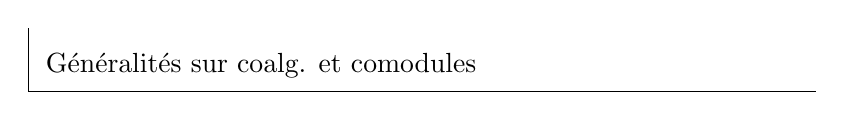
\begin{tikzpicture}\node[anchor=south west] at (.1,.05) {Généralités sur coalg. et comodules};\draw (0,.8)--(0,0)--(10,0);\end{tikzpicture}}

Soit $s$ une $k$-coalg (\deleted{\unsure{commu}}, ass \unsure{unit})
$C$ un comodule \inserted{à g.} sur $s$
donc $V_k(C)$ est un Module \inserted{\unsure{à d.}} sur $V_k(s)$ ; \deleted{\unsure{qui}} donc \inserted{l'Alg.} $V_k(s)$ opère \inserted{\unsure{à d.}} sur $V_k(C)$ ; donc l'algèbre $V_k(s)(k)=s^k$ opère \inserted{\unsure{à d.}} sur $V_k(C)$, donc à droite sur $C$. Donc $C$ est un module \inserted{à droite} ordinaire sur $s^k$, et sa structure de $k$-module s'en déduit (par $k\longrightarrow s^k$).

Quand peut-on récupérer la structure de comodule \inserted{(à g.)} sur $s$, connaissant la structure de module (à dr.) sur $s^k$ ? [NB. il est clair que si on connaît la structure de module à dr. de $C\otimes_k k'$ sur $s^{k'}$ $\forall k'$, alors on connaît la structure de comodule de $C$ sur $s$ ; de façon plus précise, une telle structure de comodule à g. \deleted{\unsure{revient}} \unsure{est la} donnée d'une structure de module, droite de
\[
W(C)=(k'\longmapsto C\otimes_k k')
\]
sous
\[
V(s)=(k'\longmapsto s^{k'}=\operatorname{Hom}_{k\text{-mod}}(s,k').
\]
] Soit $u\in s^k$, $u:s\mathbin{\text{---}}k$, alors l'op. $u_C$ de $u$ sur $C$ est le composé
\diagram{\begin{tikzcd}
C\arrow[r,"\Delta_C"]\arrow[rr,bend right=25,"u_C"'] & C\otimes s\arrow[r,"\mathrm{id}_C\otimes u"] & C\otimes k\simeq C
\end{tikzcd}}
donc la connaissance des $u_C$ équivaut à la connaissance du composé
\diagram{\begin{tikzcd}
C\arrow[r,"\Delta_C"] & C\otimes s\arrow[r,"\mathrm{id}_C\otimes u"] & \displaystyle\prod_{u\in s^k}C\otimes k
\end{tikzcd}}
et tt est bien si $C\otimes s\mathbin{\text{---}}\prod_{u\in s^k}C\otimes k$ est injectif.
\margin{152}
